%

\includegraphics[height=3.5cm]{./pics/agent-smith.jpg}

\begin{frame}
    \frametitle{Agent history}

    \begin{itemize}
        \item a fork of OCS Inventory UNIX agent by its author
        \item started 5 years ago
        \item GPLv2
    \end{itemize}
\end{frame}

\begin{frame}
    
\includegraphics[height=4.0cm]{pics/Perl_Foundation.pdf}
    \frametitle{use Perl Luke!}

    We choose to use only Perl on the agent side.
    \begin{itemize}
        \item portable
        \item reliable
        \item versatil
    \end{itemize}
\end{frame}

\begin{frame}
    \frametitle{HTTP/HTTPS}

    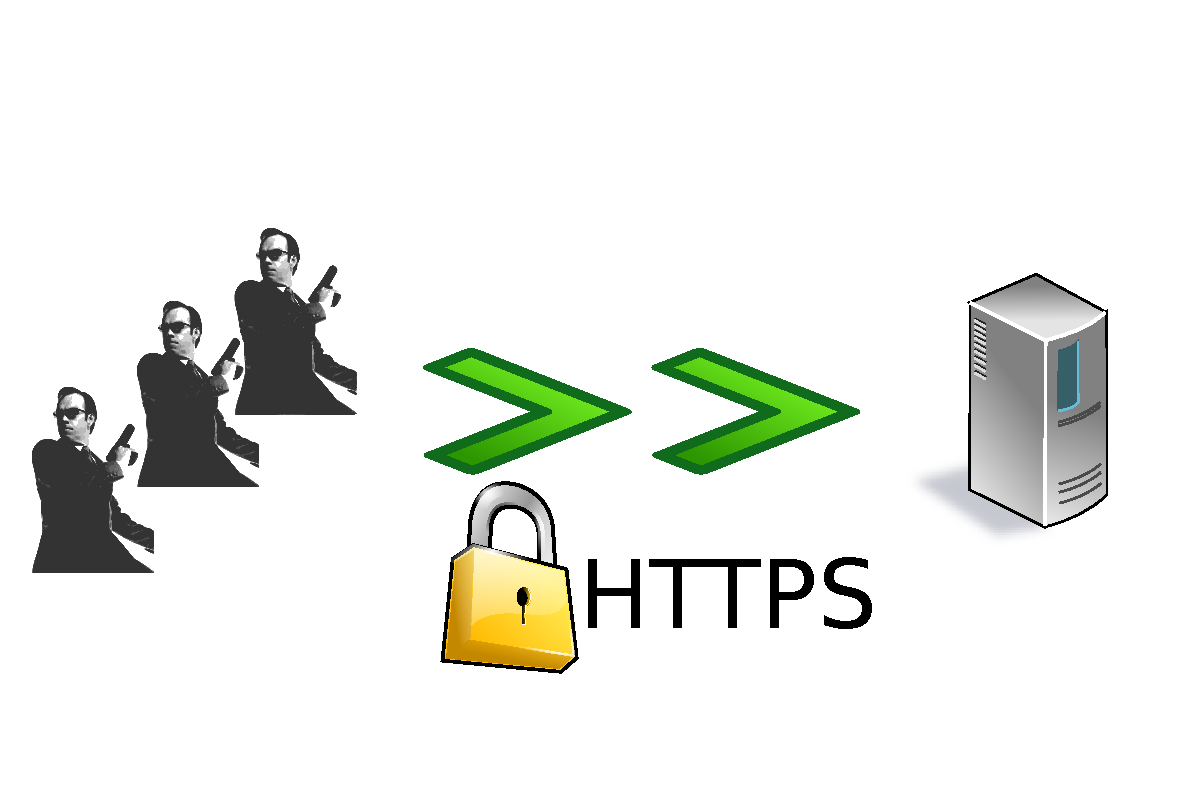
\includegraphics[height=6.0cm]{pics/https.pdf}
\end{frame}

\begin{frame}
    \frametitle{PUSH/PULL}
    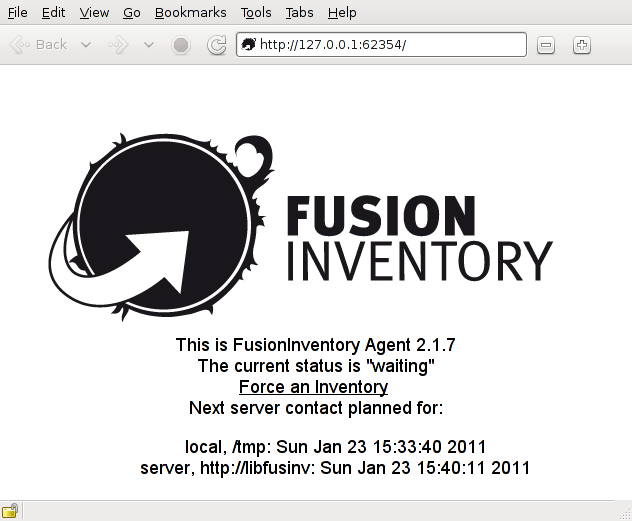
\includegraphics[height=4.0cm]{pics/http-server.png}

    thanks to an embedded http server agent get updated by the server or retrieve itself (PULL) request.
\end{frame}

\begin{frame}
    \frametitle{Task}
    %
    Not only for local machine inventory. The agent supports different "task".
\end{frame}

\begin{frame}
    \frametitle{supported OS (1/2)}
    Perl runs everywhere.
    \pause
    Basicly to do a portage of the agent we
    \begin{itemize}
        \item extend the Inventory modules to collect information
        \item and, hum, well, that's all. We're done :D
    \end{itemize}
\end{frame}

\begin{frame}
    \frametitle{supported OS (2/2)}
    Supported Operating Systems:
    \begin{itemize}
        \item<2-> Linux
        \item<3-> BSD
        \item<4-> AIX
        \item<5-> HP-UX
        \item<6-> Solaris
        \item<7-> Windows, all from 2000 to Seven 64bit
    \end{itemize}
    \uncover<8->{A complet list is avalaible on the website.}
\end{frame}
 
